\section{Templates}




\subsection{Boat}
The boat template is a model of a real boat. 
The boat is capable of carrying at most two persons and most have at least one adult to handle the boat. 
From the initial state, named Still, the only possible edge is to the OnePerson location. 
In this edge the boat calls for a handshake on the adultOn channel. 
Only persons responds to this and only one person can respond to a handshake.
A transition is made when a person responds to the handshake.  
When a person responds to the handskake the persons sailing time is transmitted through the global variable temp\_sailtime. 
This is necessary since UPPAAL does not support message parsing. 
A function set\_sailtime is used to set the sailtime to the lowest value, so the sailing time of the fastest person is the one used. 
The function set\_sailtime compares the received sail time to the one already sat on the boat. 
Temp\_sailtime is reset to reduce the state space.
From the OnePerson location there are three edges. 
Two edges to the TwoPerson location where either a child or an adult embarks. 
The adultOn edge is similar to the first edge described. 
The childOn edge does not need to synchronize a sail time since the children does not handle the boat. 
From both the TowPerson and the OnePerson location an edge to the Sailing location is possible. 
Here a guard calls the function verify, which is described in \ref{}. 
The Sailing location has an invariant that makes sure it stays in the location for at least the time it takes for the person to sail across. 
The only possible edge from the Sailing location is to the Arrived location. 
This edge has a guard to make sure that the boat arrives when it has stayed in the Sailing location in a period equivalent to the sail\_time. 
The edge broadcasts on allDisembark, which makes all persons on the boat disembark. 
The local variable boatL is fliped to note that the boat has changed site. 
After the disembarkment the sail\_time is reset to the maximum sail time and the position of the persons is verified using the verify function. 
\begin{figure}%
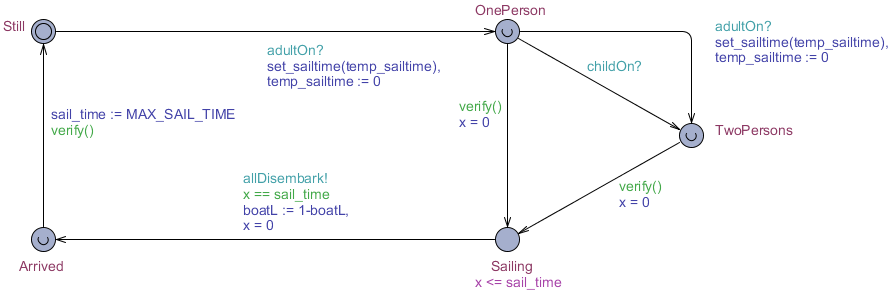
\includegraphics[width=\columnwidth]{pictures/boat.png}%
\caption{}%
\label{}%
\end{figure}
















\section{Person}
\begin{figure}%
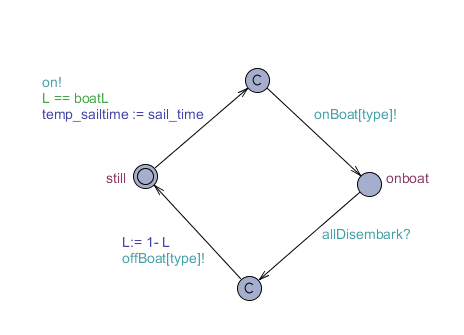
\includegraphics[width=\columnwidth]{pictures/person.png}%
\caption{}%
\label{}%
\end{figure}



















\section{Observer}
\begin{figure}%
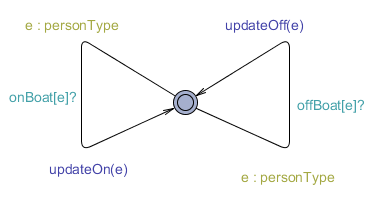
\includegraphics[width=\columnwidth]{pictures/observer.png}%
\caption{}%
\label{}%
\end{figure}




























\section{Observer}